\section{Model Evaluation}

\subsection{Advantages of the Model}%（建模方法创新、求解特色等） 

\begin{itemize}
	
	%得到满意的解
	%较好地解决了…问题
	%使模型得到简化 
	%使结果更合理，避免…带来的较大误差
	%使问题描述比较清晰
	%减少大的计算量
	
	\item[(1)] \textbf{端到端一致的数据口径与可复现流水线：}从原始DWTS宽表到周度面板与赛季特征，再到Q1--Q4所有输出均可一键再生，避免了“结果图表与模型输入不一致”的常见问题.
	
	\item[(2)] \textbf{显式表达不确定性：}Q1将观众偏好视为潜在量，通过后验抽样给出区间与稳定性诊断，使得后续机制比较不再依赖单点估计，从而提高结论可信度.
	
	\item[(3)] \textbf{机制设计的决策表达更贴近实际：}Q4将公平性（技术保护）、娱乐性（观众表达）与鲁棒性（压力测试）统一到同一坐标系，并给出可解释的推荐区域与对比可视化，便于给出可执行的制度建议.
	
\end{itemize}	

\subsection{Disadvantages of the Model}
%主观性过强
%建立在什么的前提条件下
%有一定的局限性
%存在不确定性
%有一定的偏差

\begin{itemize}
	
	\item[(1)] \textbf{观众投票的不可观测性限制：}题面数据未直接提供真实投票数/投票比例，Q1的观众偏好推断本质上依赖淘汰结果与评委信号的间接约束，仍可能存在不可辨识的等价解释.
	
	\item[(2)] \textbf{参数选择存在规范性：}例如Q4中“理想区域”的阈值（适度随机性区间与TPI阈值）反映了制作方偏好，尽管我们可通过灵敏度与压力测试展示稳健性，但无法完全消除偏好设定.
	
	\item[(3)] \textbf{外推到新赛制的假设：}在提出新机制时，我们默认观众与评委行为结构在制度改变后不会发生剧烈策略性调整；若现实中出现强策略行为，需引入博弈或行为模型进一步扩展.
	
\end{itemize}	

\subsection{Key visual evidence}
为便于评卷人在“现象---机制---决策”链路上快速核对我们的主张，我们在Q4给出两类关键图证：其一是结果不确定性的故事板（图\ref{fig:q4_champion_uncertainty_analysis}），其二是多目标权衡的机制对比散点图（图\ref{fig:q4_mechanism_tradeoff_scatter}）。

\begin{figure}[H]
	\centering
	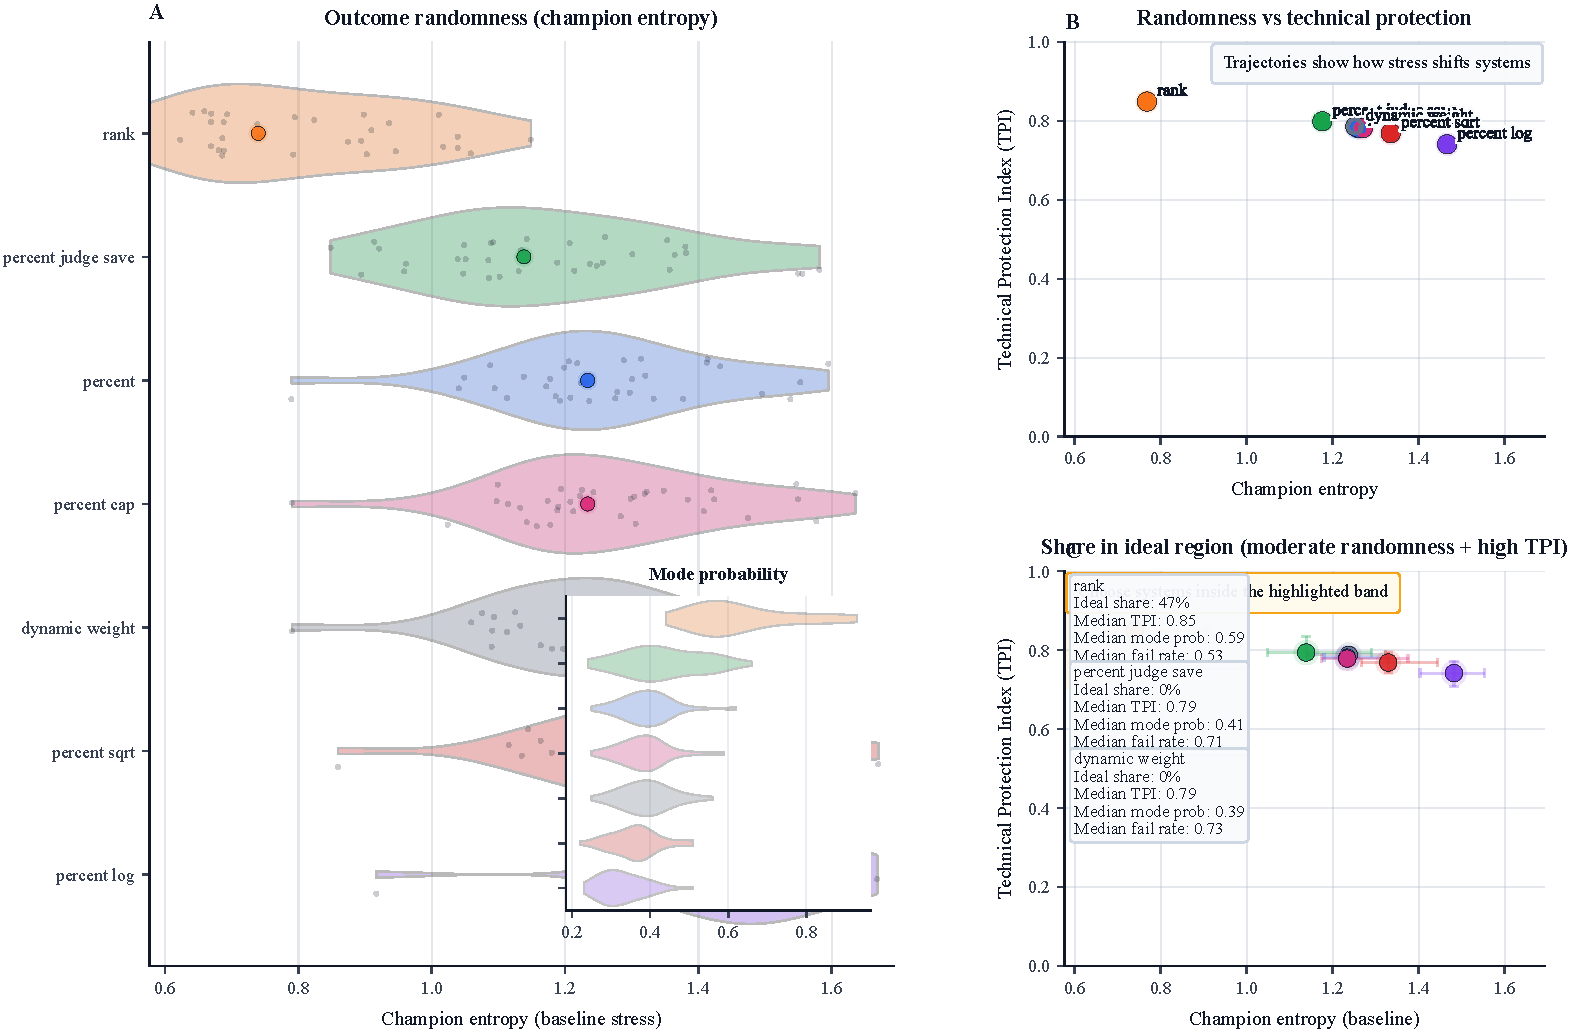
\includegraphics[width=0.98\linewidth]{../outputs/figures/q4/pdf/q4_champion_uncertainty_analysis.pdf}
	\caption{Q4冠军不确定性故事板：A显示随机性分布形状，B显示压力轨迹下随机性与技术保护的权衡，C给出推荐区域与候选机制摘要。}
	\label{fig:q4_champion_uncertainty_analysis}
\end{figure}

\begin{figure}[H]
	\centering
	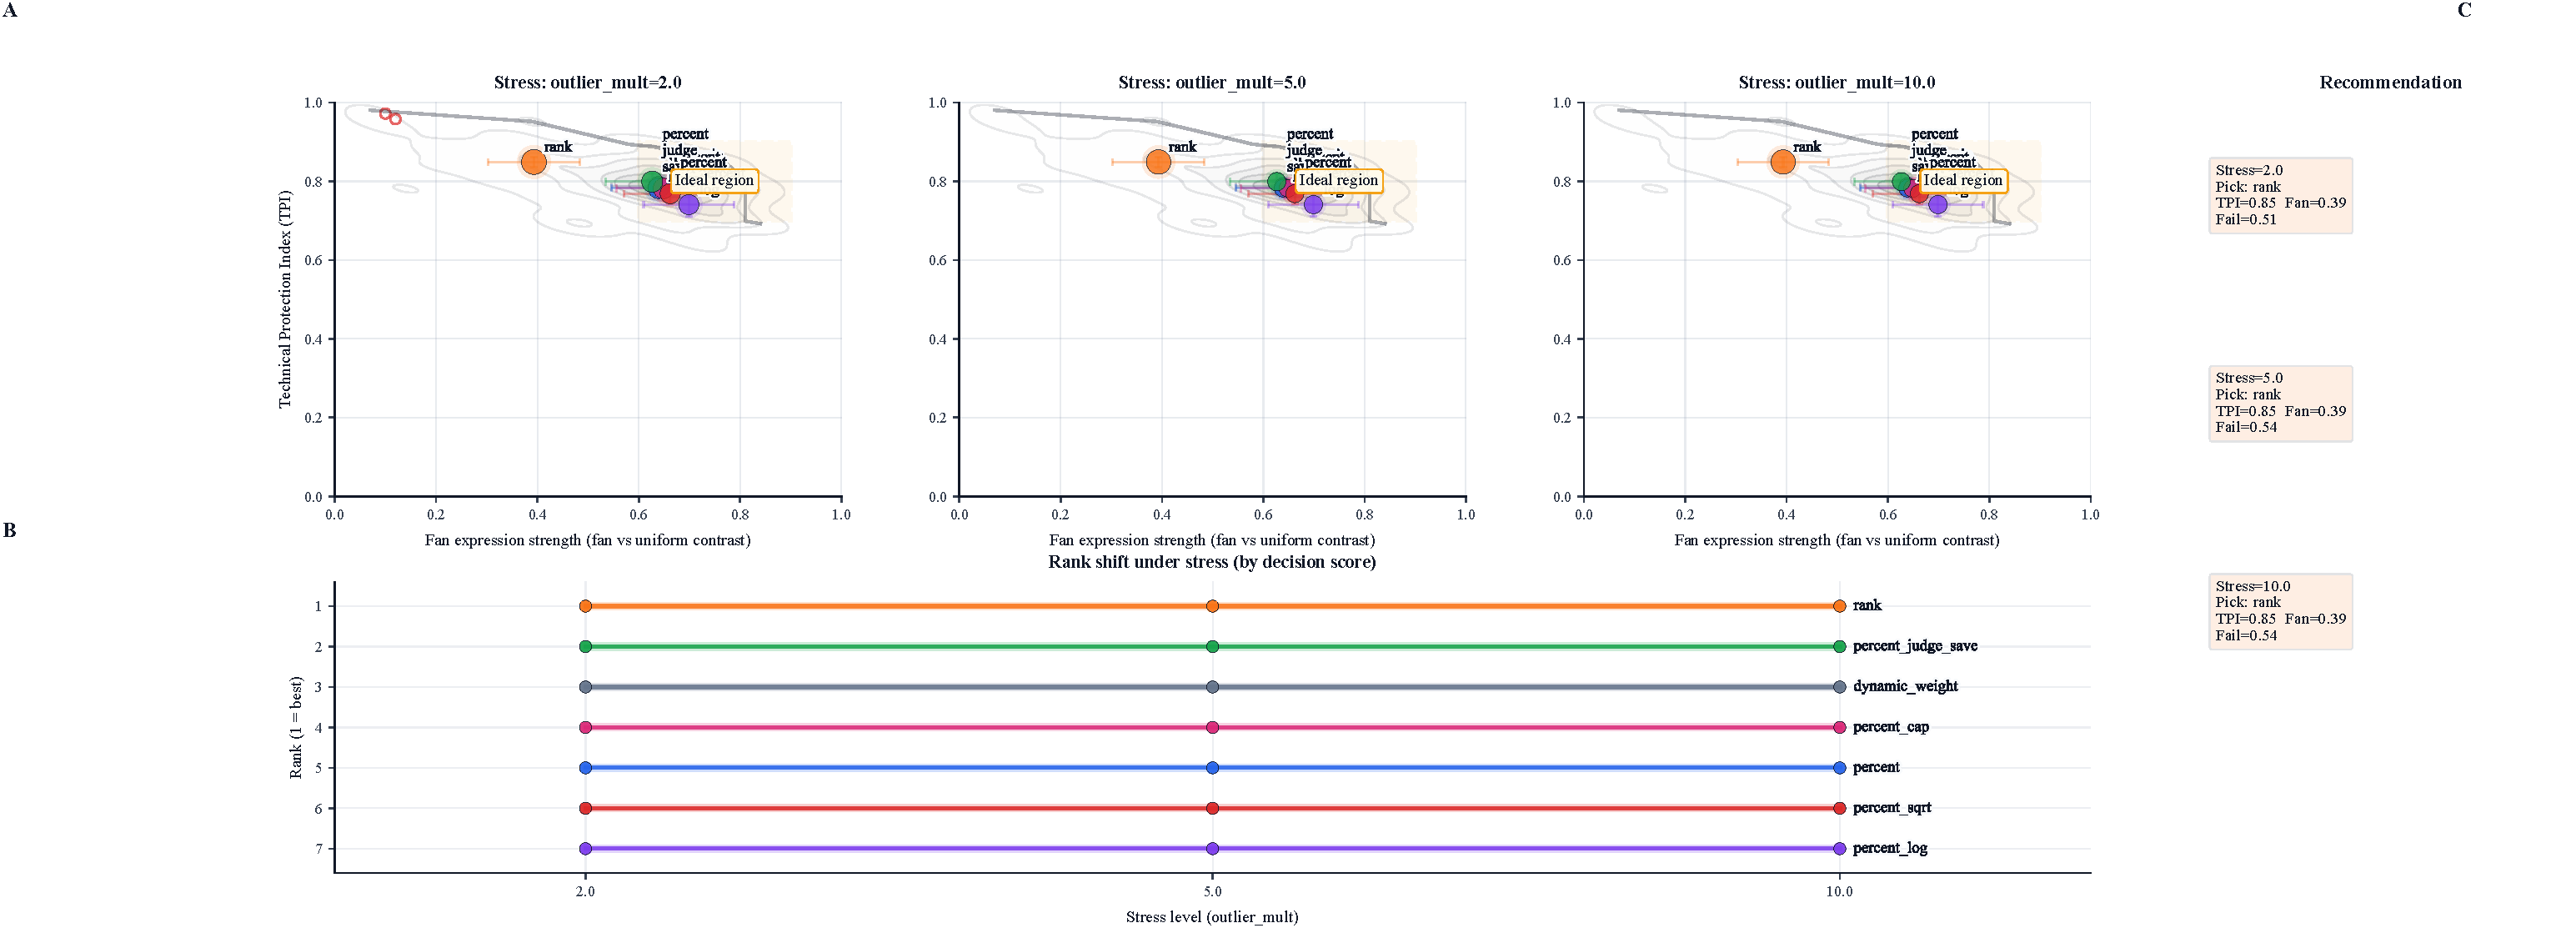
\includegraphics[width=0.98\linewidth]{../outputs/figures/q4/pdf/q4_mechanism_tradeoff_scatter.pdf}
	\caption{Q4多目标权衡：在不同压力强度下比较各机制的观众表达与技术保护，并以点大小/误差条呈现鲁棒性与不确定性。}
	\label{fig:q4_mechanism_tradeoff_scatter}
\end{figure}

为将多目标结果转化为可执行的制度建议，我们进一步给出“机制选择指南”故事板（图\ref{fig:q4_mechanism_recommendation}）：A为基线压力下的机制地图与理想区域，B为不同优先级在不同压力水平下的推荐卡片，C展示压力增加时的排名漂移，便于制作方在“偏好---压力”条件下快速选型。

\begin{figure}[H]
	\centering
	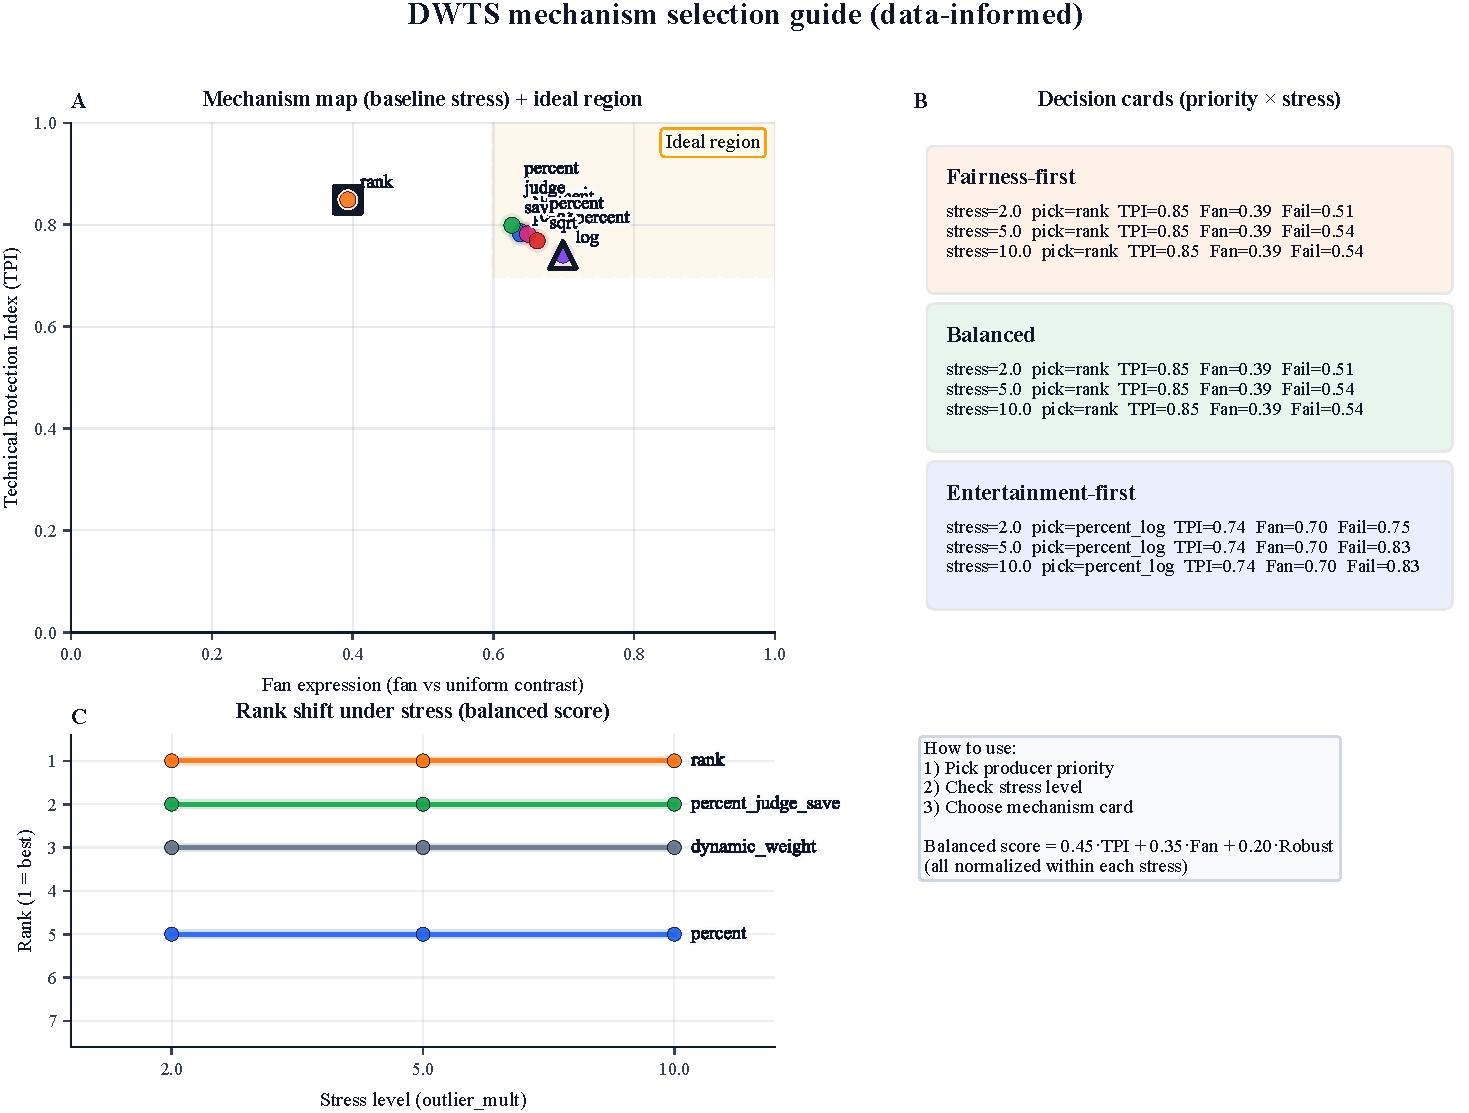
\includegraphics[width=0.98\linewidth]{../outputs/figures/q4/pdf/q4_mechanism_recommendation.pdf}
	\caption{Q4机制推荐故事板：将公平性、娱乐性与鲁棒性统一到决策视图中，并给出不同优先级与压力水平下的推荐机制。}
	\label{fig:q4_mechanism_recommendation}
\end{figure}

\section{Conclusion} %总结与展望